\chapter{Week}
The first two days of the week were spent getting to know all colleagues and familiarize myself with internal processes and guidelines. Zurich is the headquarters of Enclustra GmbH and therefore the majority of hardware and software design is being done here. Around forty people, most of which are hardware and software engineers, work in the Zurich office. The company itself is divided into two areas, \ac{FPGA} Design Center and \ac{FPGA} Solution Center.
The former is offering customer-specific design services implementing applications on \acp{FPGA} and providing support and custom \ac{IP} components. Areas of expertise include wired networks and switching, wireless communications (\ac{SDR}), smart cameras, embedded interfaces (\ac{PCIe}, \ac{USB}, \ac{AXI}, ethernet, etc.), test and measurement (sensors, data acquisition, \ac{DSP}) and drive/motion control. 
The latter designs custom \ac{FPGA}/\ac{SoC} modules and \ac{IP} solutions. Several base board families and \ac{FPGA} module families are developed and supported which can be adapted to the needs of the application by offering different performance key points. Reference designs for each combination of base board and module are provided as a starting point for customers.
Furthermore, my task was to do market research on artificial intelligence and artificial intelligence on \acp{FPGA} especially. The four key platforms for artificial neural network applications are shown in~\ref{fig:overview}.
\begin{figure}[!htb]
	\centering
		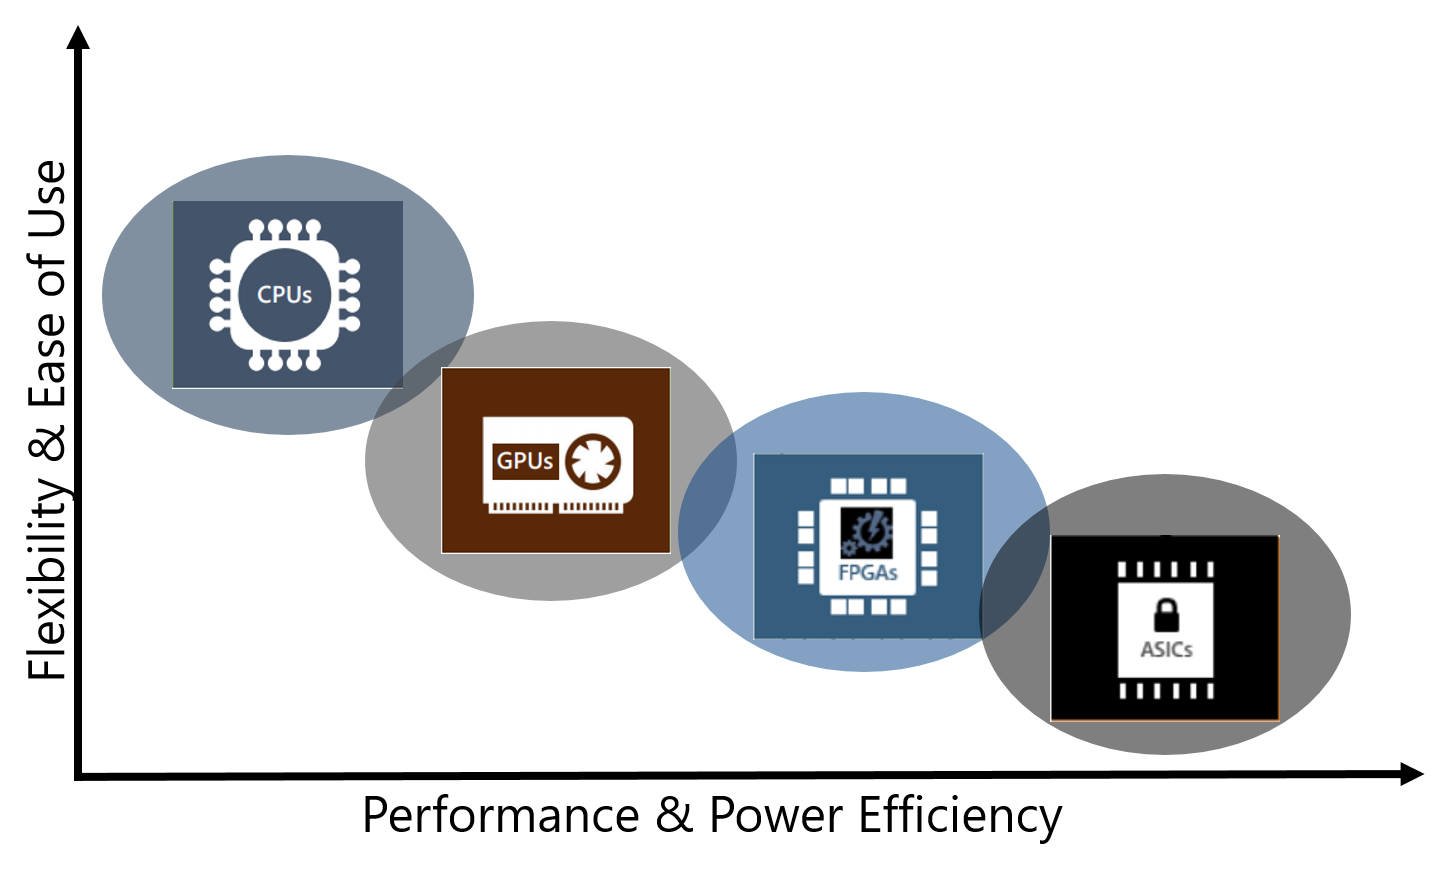
\includegraphics[width=0.75\textwidth]{bilder/overview.png}
		\caption{Hardware platform overview}
		\label{fig:overview}
\end{figure}
A qualitative design trade-off is shown on the $x$- and $y$-axis in terms of power efficiency and performance versus flexibility and ease-of-use. As Enclustras focus is on the embedded market, the market survey has been mainly on \acp{GPU}, \acp{FPGA} and \acp{ASIC} as full blown \acp{CPU} are too inefficient for embedded applications. Possible competitors as well as toolkits provided by \ac{FPGA} manufacturers such as Intel, Xilinx and Lattice have been evaluated. The results have been presented in a meeting in which a discussion has been held, where Enclustras products and services can fit. One of the results was to start planning an \ac{AI} demonstrator using Enclustra hardware. The purpose of this demonstrator was to showcase machine learning applications running on Enclustra hardware. As a preliminary step it was decided to check the Xilinx \ac{DNNDK} samples on an evaluation board, the ZCU 104.